\pdfoutput=1
\pdfcompresslevel=9
\documentclass[a4paper,onecolumn,oneside,11pt,wide,floatssmall]{mwrep}
\usepackage{algorithm}
\usepackage{algpseudocode}
\usepackage{amsmath}
\usepackage{amsfonts}
\usepackage{amssymb}
\usepackage{amsthm}
\usepackage{float}
\usepackage{geometry}
\usepackage{listings}
\usepackage[pdftex]{color,graphicx}
\usepackage[polish]{babel}
\usepackage[pdftex, bookmarks=false]{hyperref}
\usepackage[T1]{fontenc}
\usepackage[utf8x]{inputenc}
\usepackage[sort, compress]{cite}

\def\url#1{{ \tt #1}}
\def\C{{\rm C}\,}
\def\E{{\rm E}\,}

% marginesy
\textwidth\paperwidth
\advance\textwidth -55mm
\oddsidemargin-0.9in
\advance\oddsidemargin 33mm
\evensidemargin-0.9in
\advance\evensidemargin 33mm
\topmargin -1in
\advance\topmargin 25mm
\setlength\textheight{48\baselineskip}
\addtolength\textheight{\topskip}
\marginparwidth15mm

\clubpenalty=10000 % to kara za sierotki
\widowpenalty=10000 % nie pozostawia wdów
\brokenpenalty=10000 % nie dzieli wyrazów pomiędzy stronami
\sloppy

\tolerance4500
\pretolerance250
\hfuzz=1.5pt
\hbadness1450

% ŻYWA PAGINA
\renewcommand{\chaptermark}[1]{\markboth{\scshape\small\bfseries \
#1}{\small\bfseries \ #1}}
\renewcommand{\sectionmark}[1]{\markboth{\scshape\small\bfseries\thesection.\
#1}{\small\bfseries\thesection.\ #1}}
\newcommand{\headrulewidth}{0.5pt}
\newcommand{\footrulewidth}{0.pt}
\pagestyle{uheadings}

\theoremstyle{definition}
\newtheorem{defn}{Definicja}[section]
\newtheorem{conj}{Teza}[section]
\newtheorem{conjmain}{Teza}
\newtheorem{exmp}{Przykład}[section]

\theoremstyle{plain}% default
\newtheorem{thm}{Twierdzenie}[section]
\newtheorem{lem}[thm]{Lemat}
\newtheorem{prop}[thm]{Hipoteza}
\newtheorem*{cor}{Wniosek}

\theoremstyle{remark}
\newtheorem*{rem}{Uwaga}
\newtheorem*{note}{Uwaga}
\newtheorem{case}{Przypadek}

\definecolor{ListingBackground}{rgb}{0.95,0.95,0.95}

\begin{document}

\renewcommand*\lstlistingname{Wydruk}
\renewcommand*\lstlistlistingname{Spis wydruków}

\pagenumbering{roman}
\renewcommand{\baselinestretch}{1.0}
\raggedbottom
\begin{titlepage}
    % Strona tytułowa
    \vbox to\textheight{\hyphenpenalty=10000
    \begin{center}
	\begin{tabular}{p{107mm} p{9cm}}
	    \begin{minipage}{9cm}
	      \begin{center}
	      Politechnika Warszawska \\
	      Wydział Elektroniki i~Technik Informacyjnych \\
	      Instytut Informatyki
	      \end{center}
	    \end{minipage}
	    &
	    \begin{minipage}{8cm}
	    \begin{flushleft}
	     \footnotesize
	      Rok akademicki 2013/2014
	    \vspace*{2.75\baselineskip}
	    \end{flushleft}
	    \end{minipage} \\
	\end{tabular}
	\vspace*{3.75\baselineskip}
	\par\vspace{\smallskipamount}
	\vspace*{2\baselineskip}{\LARGE Praca dyplomowa magisterska\par}
	\vspace{3\baselineskip}{\LARGE\strut Adam Stelmaszczyk\par}
	\vspace*{2\baselineskip}{\huge\bfseries DE/mid -- nowy wariant algorytmu ewolucji różnicowej wykorzystujący punkt środkowy populacji\par}

	\vspace*{2\baselineskip}
	\hfill\mbox{}\par\vspace*{\baselineskip}\noindent
	\begin{tabular}[b]{@{}p{3cm}@{\ }l@{}}
	    {\large\hfill } & {\large }
	\end{tabular}
	\hfill
	\begin{tabular}[b]{@{}l@{}}
	Opiekun pracy: \\[\smallskipamount]
	{\large prof. nzw. dr hab. Jarosław Arabas}
	\end{tabular}\par
	\vspace*{2\baselineskip}
    \begin{tabular}{p{\textwidth}}
    \begin{flushleft}
	\begin{minipage}{7cm}
	Ocena \dotfill
	\par\vspace{1.6\baselineskip}
	\dotfill
	\par\noindent
	\centerline{\footnotesize Podpis Przewodniczącego} \par
	\centerline{\footnotesize Komisji Egzaminu Dyplomowego}\par
	\end{minipage}
    \end{flushleft}
    \end{tabular}
    \end{center}}

    % Życiorys
    \newpage\thispagestyle{empty}
    \begin{tabular}{p{5cm} p{12cm}}
    \begin{minipage}{5cm}
    \center
    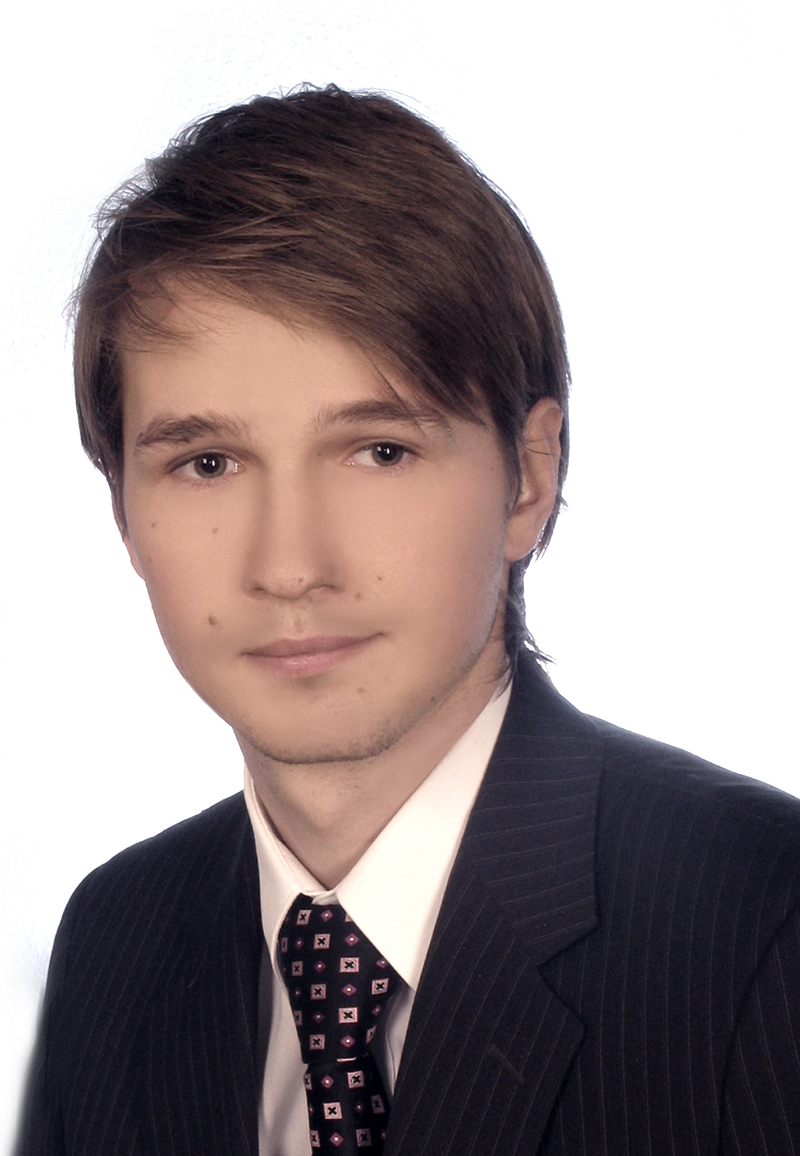
\includegraphics[height=6.5cm,width=4.5cm]{img/foto.jpg}
    \end{minipage}
    &
    \begin{minipage}{12cm}
    \begin{flushleft}
    \par\noindent\vspace{1\baselineskip}
    \begin{tabular}[h]{l l}
    {\normalsize\it Specjalność:} & \normalsize Inżynieria Systemów Informacyjnych 
    \end{tabular}
    \par\noindent\vspace{1\baselineskip}
    \begin{tabular}[h]{l l}
    {\normalsize\it Data urodzenia:} & {\normalsize 12 stycznia 1990~r.}
    \end{tabular}
    \par\noindent\vspace{1\baselineskip}
    \begin{tabular}[h]{l l}
    {\normalsize\it Data rozpoczęcia studiów:} & {\normalsize 1 października 2009 r.}
    \end{tabular}
    \par\noindent\vspace{1\baselineskip}
    \end{flushleft}
    \end{minipage}
    \end{tabular}
    \vspace*{1\baselineskip}
    \begin{center}
	{\large\bfseries Życiorys}\par\bigskip
    \end{center}

    \indent
Urodziłem się 12 stycznia 1990 roku w Piotrkowie Trybunalskim. Ukończyłem Szkołę Podstawową
nr 33, Gimnazjum nr 11 oraz Liceum Ogólnokształcące im. Jana Kochanowskiego w Warszawie, gdzie
uczęszczałem do klasy o profilu matematyczno--fizyczno--informatycznym.
W październiku 2009 roku rozpocząłem studia na Wydziale Elektroniki i Technik Informacyjnych
Politechniki Warszawskiej na kierunku Informatyka. W lutym 2013 roku uzyskałem tytuł inżyniera.

    \par
    \vspace{3\baselineskip}
    \hfill\parbox{15em}{{\small\dotfill}\\[-.3ex]
    \centerline{\footnotesize podpis studenta}}\par
    \vspace{2\baselineskip}
    \begin{center}
 	{\large\bfseries Egzamin dyplomowy} \par\bigskip
    \end{center}
    \par\noindent\vspace{1\baselineskip}
    Złożył egzamin dyplomowy w dn. \dotfill
    \par\noindent\vspace{1\baselineskip}
    Z wynikiem \dotfill
    \par\noindent\vspace{1\baselineskip}
    Ogólny wynik studiów \dotfill
    \par\noindent\vspace{1\baselineskip}
    Dodatkowe wnioski i uwagi Komisji \dotfill
  
    % Streszczenie
    \newpage\thispagestyle{empty}
    \vspace*{2\baselineskip}
    \begin{center}
	{\large\bfseries Streszczenie}\par\bigskip
    \end{center}

    {\itshape
W pracy przeanalizowano działanie znanych wariantów algorytmu ewolucji różnicowej~--~DE/rand
oraz DE/best. W celu poprawienia wyników zaproponowano nowy wariant nazwany DE/mid. 
Żeby porównanie jakości algorytmów było sprawiedliwe, każdemu z wariantów ustalono taki sam zasięg
mutacji poprzez dobranie odpowiedniego współczynnika skalującego.
Na podstawie przeprowadzonych testów stwierdzono poprawę jakości uzyskiwanych wyników na 6 z 7 
wielowymiarowych funkcji testowych z zestawu BBOB 2013.}
    \vspace*{1\baselineskip}

    \noindent{\bf Słowa kluczowe}: {\itshape ewolucja różnicowa, algorytm ewolucyjny, genetyczny, optymalizacja globalna}
    \par
    \vspace{4\baselineskip}
    \begin{center}
	{\large\bfseries Abstract}\par\bigskip
    \end{center}
    \noindent{\bf Title}: {\itshape DE/mid -- new variant of differential evolution algorithm using the midpoint of the population}\par
    \vspace*{1\baselineskip}
    {\itshape
This thesis analyzes behaviour of known differential evolution variants -- DE/rand and DE/best.
In order to achieve better performance, new variant named DE/mid has been introduced.
To ensure a fair comparison between algorithms, mutation of every algorithm variant had exactly
the same range. 
Tests indicated improvement of results quality on 6 out of 7 high-dimensional
testing functions from BBOB 2013 testbed.}
    \vspace*{1\baselineskip}

    \noindent{\bf Key words}: {\itshape differential evolution, evolutionary, genetic algorithm, global optimization
}

\end{titlepage}

\tableofcontents

\newpage
\pagenumbering{arabic}
\setcounter{page}{1}

\chapter{Wprowadzenie}

\section{Część teoretyczna}

Klasyczna ewolucja różnicowa DE/rand oraz jej odmiana DE/mid różnią się jedynie operatorem mutacji.
W poniższych rozdziałach przedstawiono operatory mutacji dla DE/rand/k, DE/mid/k, DE/rand/$\infty$, DE/mid/$\infty$
oraz wyprowadzono wzory na współczynniki skalujące.

\subsection{Mutacja w DE/rand}

W DE/rand/1, mutant $i$-tego osobnika w populacji $P$~o~$n$~osobnikach powstaje w następujący sposób \cite{opara}:
\begin{equation} \label{eq:derand1}
u_i = P_{i_1} + F(P_{i_2} - P_{i_3})
\end{equation}

$i_1, i_2, i_3$ to indeksy wylosowane zgodnie z rozkładem jednostajnym ze zbioru \\ 
$\{0, 1, \dots, n-1\}$. Zatem $P_{i_1}, P_{i_2}, P_{i_3}$ to rozwiązania wylosowane zgodnie z rozkładem jednostajnym z populacji $P$.
$F\in\mathbb{R_+}$ to współczynnik skalujący, w tej pracy ustalony na 0,9. \\

DE/rand/1 można uogólnić na DE/rand/k, w którym to dodajemy
$k \in \mathbb{N}$ wektorów różnicowych:
\begin{equation} \label{eq:derand}
u_i' = P_{i_1} + F_k\sum\limits_{j=1}^k (P_{i_{2j}} - P_{i_{2j+1}})
\end{equation}

Podobnie jak poprzednio, $i_1, i_2, \dots i_{2k+1}$ to indeksy wylosowane zgodnie z rozkładem jednostajnym ze zbioru 
$\{0, 1, \dots, n-1\}$. Zatem $P_{i_1}, P_{i_2}, \dots, P_{2k+1}$ to rozwiązania wylosowane zgodnie z rozkładem 
jednostajnym z populacji $P$. $F_k\in\mathbb{R_+}$ to współczynnik skalujący dla DE/rand/k. 
Żeby macierz kowariancji populacji w DE/rand/k nie zmieniała się wraz z zmianą $k$, 
macierz kowariancji mutanta $u_i'$ musi być taka sama jak macierz kowariancji mutanta $u_i$.
Można to osiągnąć tak dobierając $F_k$, aby było spełnione równanie:
\begin{equation} \label{eq:kowariancje}
\C[u_i] = \C[u_i']
\end{equation}

Osobniki są liniowo niezależne od siebie, dlatego:
\begin{align*}
\C[u_i] \overset{(\ref{eq:derand1})}{=} \C[P_{i_1} + F(P_{i_2} - P_{i_3})] = \C[P_{i_1}] + F^2(\C[P_{i_2}] + \C[P_{i_3}])
\end{align*}

$\forall{i}\hspace{1mm}\C[P_i] = \C[P]$, ponieważ każdy osobnik ma taki sam rozkład prawdopodobieństwa. Zatem:
\begin{equation} \label{eq:macierz_kow_mutanta}
\C[u_i] = \C[P] + F^2(\C[P] + \C[P]) = \C[P](2F^2 + 1)
\end{equation}

Rozwijając prawą stronę równania (\ref{eq:kowariancje}):
\begin{align*}
\C[u_i'] \overset{(\ref{eq:derand})}{=} \C[P_{i_1} + F_k\sum\limits_{j=1}^k (P_{i_{2j}} - P_{i_{2j+1}})] 
= \C[P_{i_1}] + F_k^2\C[\sum\limits_{j=1}^k (P_{i_{2j}} - P_{i_{2j+1}})] \\
= \C[P_{i_1}] + F_k^2\C[\sum\limits_{j=2}^{2k+1} P_{i_{j}}] \\
= \C[P](2kF_k^2 + 1)
\end{align*}

Podstawiając do (\ref{eq:kowariancje}):
\begin{align*}
\C[P](2F^2 + 1) = \C[P](2kF_k^2 + 1)
\end{align*}

Zakładając, że $\C[P] \neq \textbf{0}$:
\begin{align*}
F^2 = kF_k^2
\end{align*}

Obie strony są nieujemne, więc ostatecznie:
\begin{align*}
F_k = \frac{F}{\sqrt{k}}
\end{align*}

\subsection{Mutacja w DE/mid}

W DE/mid/k mutant powstaje w następujący sposób:

\begin{equation} \label{eq:demid}
u_i'' = m + F_m\sum\limits_{j=1}^k (P_{i_{2j}} - P_{i_{2j+1}})
\end{equation}

Jedyną różnicą w porównaniu do DE/rand/k jest $m$, czyli punkt środkowy populacji:
\begin{equation} \label{eq:midpoint}
m = \frac{1}{n}\sum\limits_{j=1}^n P_j
\end{equation}

$F_m\in\mathbb{R_+}$ jest współczynnikiem skalującym dla DE/mid/k, analogicznym do $F$ dla DE/rand/1. 
Żeby macierz kowariancji populacji w DE/mid była taka sama jak w DE/rand/1, 
macierz kowariancji mutanta $u_i''$ musi być taka sama jak macierz kowariancji mutanta $u_i$.
Można to osiągnąć tak dobierając $F_m$, żeby było spełnione równanie:
\begin{equation} \label{eq:rownanie}
\C[u_i] = \C[u_i'']
\end{equation}

Rozwijając prawą stronę równania (\ref{eq:rownanie}):
\begin{align*}
\C[u_i''] \overset{(\ref{eq:demid})}{=} \C[m + F_m\sum\limits_{j=1}^k (P_{i_{2j}} - P_{i_{2j+1}})] \\
\overset{(\ref{eq:midpoint})}{=} \C[\frac{1}{n}\sum\limits_{j=1}^n P_j] + F_m^2\C[\sum\limits_{j=1}^k (P_{i_{2j}} - P_{i_{2j+1}})] 
= \frac{1}{n^2}n\C[P] + F_m^2\C[\sum\limits_{j=2}^{2k+1} P] = \C[P](2kF_m^2 + \frac{1}{n})
\end{align*}

Podstawiając do (\ref{eq:rownanie}):
\begin{align*}
\C[P](2F^2 + 1) = \C[P](2kF_m^2 + \frac{1}{n})
\end{align*}

Przy założeniu, że $\C[P] \neq \textbf{0}$:
\begin{align*}
2F^2 + 1 = 2kF_m^2 + \frac{1}{n} \\
F_m^2 = \frac{2F^2 + 1 - \frac{1}{n}}{2k}
\end{align*}

Obie strony są nieujemne, więc:
\begin{align} \label{eq:a}
F_m\ = \sqrt{\frac{2F^2 + 1 - \frac{1}{n}}{2k}}
\end{align}

Przyjmując $F=0,9$ z (\ref{eq:a}) wynika, że: \\
$F_m \approx 1,14$ dla $k=1$ i $n\to\infty$. \\

W DE/mid przesuwany jest punkt środkowy $m$ zamiast losowo wybranego osobnika $P_{i_1}$.
Punkt środkowy jest mniej zmienny, 
tzn. norma macierzy kowariancji punktu środkowego jest mniejsza niż norma macierzy kowariancji dowolnego osobnika.
$\lim_{n\to\infty} \C[m] = \textbf{0}$, natomiast $\C[P_{i_1}] = \C[P]$.
Dlatego DE/mid/k potrzebuje większego współczynnika skalującego niż DE/rand/k. \\

\subsection{Mutacja w DE/rand/$\infty$}

Zgodnie z centralnym twierdzeniem granicznym, $\frac{1}{{\sqrt{k}}}\sum\limits_{j=1}^k (P_{i_{2j}} - P_{i_{2j+1}})$ 
zbiega według rozkładu do $\mathcal{N}(0, \C[P])$ gdy $k \to \infty$. 
Dzięki temu, równanie mutanta DE/rand/$\infty$ można zapisać jako:
\begin{align*}
u_i = P_{i_1} + F_\infty \cdot v_\infty
\end{align*}

Gdzie $v_\infty \sim \mathcal{N}(0, \C[P])$. Wyznaczmy $F_\infty$.
\begin{align*}
\C[u_i] = \C[P_{i_1} + F_\infty \cdot v_\infty] \overset{(\ref{eq:macierz_kow_mutanta})}{=} \C[P](2F^2 + 1) \\
\C[P] + \C[F_\infty \cdot v_\infty] = \C[P](2F^2 + 1) \\
\C[F_\infty \cdot v_\infty] = 2F^2\C[P] \\
F_\infty^2 \C[P] = 2F^2\C[P] \\
F_\infty^2 = 2F^2 \\
F_\infty = \sqrt{2}F
\end{align*}

\subsection{Mutacja w DE/mid/$\infty$}

Równanie mutanta DE/mid/$\infty$ można zapisać podobnie:
\begin{align*}
u_i' = m + F_{\infty_m} \cdot v_\infty
\end{align*}

Wyznaczmy $F_{\infty_m}$.
\begin{align*}
\C[u_i'] = \C[m + F_{\infty_m} \cdot v_\infty] \overset{(\ref{eq:macierz_kow_mutanta})}{=} \C[P](2F^2 + 1) \\
\C[m] + C[F_{\infty_m} \cdot v_\infty] = \C[P](2F^2 + 1) \\
\frac{C[P]}{n} + F_{\infty_m}^2 C[P] = \C[P](2F^2 + 1) \\
F_{\infty_m} = \sqrt{2F^2 + 1 - \frac{1}{n}}
\end{align*}

\subsection{Podsumowanie}

Tabela \ref{table:parametry} podsumowuje znalezione współczynniki skalujące.

\begin{table}[H]
\centering
\begin{tabular}{ l | l }
algorytm         & współczynnik \\ \hline
DE/rand/k        & $\sqrt{\frac{2F^2}{2k}} = \frac{F}{\sqrt{k}}$ \\ 
DE/rand/$\infty$ & $\sqrt{2F^2} = \sqrt{2}F$ \\ \hline
DE/mid/k         & $\sqrt{\frac{2F^2 + 1 - \frac{1}{n}}{2k}}$ \\
DE/mid/$\infty$  & $\sqrt{2F^2 + 1 - \frac{1}{n}}$ \\
\end{tabular}
\caption{Współczynniki skalujące}
\label{table:parametry}
\end{table}

\section{Część praktyczna}

Przetestowano 8 algorytmów:

\begin{enumerate}
 \item DE/rand/1
 \item DE/rand/2
 \item DE/rand/6
 \item DE/rand/$\infty$ 
 \item DE/mid/1 
 \item DE/mid/2
 \item DE/mid/6 
 \item DE/mid/$\infty$ 
\end{enumerate} 

Eksperymenty przeprowadzono na 7 funkcjach testowych o numerach 15, 16, 19, 20, 21, 22, 24 z BBOB 2013 \cite{finck}, zaimplementowanych w języku C.
Funkcje testowe są wywoływane z Javy, w której napisano algorytmy oraz procedurę testującą.
Liczba wymiarów $D \in \{10, 20, 40, 80\}$. Maksymalna liczba wywołań funkcji oceny $FEs = 10^5D$. Rozmiar populacji $n = 10D$. 
Jeśli algorytm nie znajdował minimum, wówczas w jednym uruchomieniu, na jednej funkcji, generował $\frac{FEs}{n} = 10^4$ pokoleń.
Na każdej funkcji algorytm był niezależnie uruchamiany 15 razy, z każdego uruchomienia zapisywany był najlepszy wynik.
$F = 0,9$. Krzyżowanie wymieniające (DE/*/k/bin).
Prawdopodobieństwo krzyżowania $Cr = 0,9$. \\

W celu porównania, wykreślono dystrybuanty empiryczne najlepszych wyników z każdego uruchomienia 
dla wszystkich algorytmów na jednej funkcji. Wykresy przedstawiono poniżej.
Najlepszym wynikiem była najmniejsza odległość funkcji oceny osobnika od minimum.
Algorytm, którego dystrybuanta na wykresie przebiegała powyżej pozostałych, otrzymywał 7 punktów. 
Za drugie miejsce algorytm otrzymywał 6 punktów, za trzecie 5 itd. Za ostatnie 0. 
Jeśli dystrybuanty się przecinały, algorytmy zajmowały i-te miejsce ex aequo i punkty były rozdzielane
po równo. 
Przykładowo, na 15 funkcji w 10 wymiarach, DE/rand/1 i DE/mid/2 zajęły ex aequo drugie miejsce,
dostając po $\frac{6+5}{2} = 5,5$ pkt.

\subsection{10 wymiarów}

W 10 wymiarach na 3 z 7 funkcji, wyniki algorytmów nie różniły się w sposób znaczący od siebie.
Na pozostałych funkcjach DE/mid/1 oraz DE/rand/1 spisały się najlepiej. DE/mid/2 dorównał DE/rand/1
na funkcji 15, przez co zajął trzecie miejsce w ogólnym rozrachunku. 

\begin{table}[H]
\centering
\begin{tabular}{ l | c | c | c | c | c | c | c | c}
                 & 15  & 16  & 19  & 20  & 21  & 22  & 24  & suma \\ \hline
DE/rand/1        & 5,5 & 7   & 3   & 7   & 3,5 & 3,5 & 3,5 & 33   \\ 
DE/rand/2        & 2   & 2,5 & 3   & 3   & 3,5 & 3,5 & 3,5 & 21   \\ 
DE/rand/6        & 2   & 2,5 & 3   & 3   & 3,5 & 3,5 & 3,5 & 21   \\ 
DE/rand/$\infty$ & 2   & 2,5 & 3   & 3   & 3,5 & 3,5 & 3,5 & 21   \\ 
DE/mid/1         & 7   & 6   & 7   & 3   & 3,5 & 3,5 & 3,5 & 33,5 \\
DE/mid/2         & 5,5 & 2,5 & 3   & 3   & 3,5 & 3,5 & 3,5 & 24,5 \\
DE/mid/6         & 2   & 2,5 & 3   & 3   & 3,5 & 3,5 & 3,5 & 21   \\ 
DE/mid/$\infty$  & 2   & 2,5 & 3   & 3   & 3,5 & 3,5 & 3,5 & 21   \\
\end{tabular}
\caption{Porównanie algorytmów w 10 wymiarze}
\label{table:10d}
\end{table}

\begin{figure}[H]
\centering
\mbox{
\includegraphics[width=.45\textwidth]{../pngs/10/15.png} \quad
\includegraphics[width=.45\textwidth]{../pngs/10/16.png} 
}
\end{figure}

\begin{figure}[H]
\centering
\mbox{
\includegraphics[width=.45\textwidth]{../pngs/10/19.png} \quad
\includegraphics[width=.45\textwidth]{../pngs/10/20.png} 
}
\end{figure}

\begin{figure}[H]
\centering
\mbox{
\includegraphics[width=.45\textwidth]{../pngs/10/21.png} \quad
\includegraphics[width=.45\textwidth]{../pngs/10/22.png} 
}
\end{figure}

\begin{figure}[H]
\centering
\mbox{
\includegraphics[width=.45\textwidth]{../pngs/10/24.png}
}
\end{figure}

\subsection{20 wymiarów}

W 20 wymiarach DE/rand/1 zdołał zremisować z DE/mid/1 na funkcji 19,
przez co w ostatecznym rankingu objął nad nim sześciopunktową przewagę.
Na trzecim miejscu ex aequo DE/mid/2 oraz DE/rand/2. Na funkcji 21 oraz 24 
nie było już ogólnego remisu, lepsze algorytmy wyszły na prowadzenie.

\begin{table}[H]
\centering
\begin{tabular}{ l | c | c | c | c | c | c | c | c}
                 & 15  & 16  & 19  & 20  & 21  & 22  & 24  & suma \\ \hline
DE/rand/1        & 6,5 & 7   & 6,5 & 7   & 6   & 3,5 & 7   & 43,5 \\ 
DE/rand/2        & 2   & 2,5 & 2,5 & 3   & 6   & 3,5 & 4   & 23,5 \\ 
DE/rand/6        & 2   & 2,5 & 2,5 & 3   & 2   & 3,5 & 1,5 & 17   \\ 
DE/rand/$\infty$ & 2   & 2,5 & 2,5 & 3   & 2   & 3,5 & 1,5 & 17   \\ 
DE/mid/1         & 6,5 & 6   & 6,5 & 3   & 6   & 3,5 & 6   & 37,5 \\
DE/mid/2         & 5   & 2,5 & 2,5 & 3   & 2   & 3,5 & 5   & 23,5 \\
DE/mid/6         & 2   & 2,5 & 2,5 & 3   & 2   & 3,5 & 1,5 & 17   \\ 
DE/mid/$\infty$  & 2   & 2,5 & 2,5 & 3   & 2   & 3,5 & 1,5 & 17   \\
\end{tabular}
\caption{Porównanie algorytmów w 20 wymiarze}
\label{table:20d}
\end{table}

\begin{figure}[H]
\centering
\mbox{
\includegraphics[width=.45\textwidth]{../pngs/20/15.png} \quad
\includegraphics[width=.45\textwidth]{../pngs/20/16.png} 
}
\end{figure}

\begin{figure}[H]
\centering
\mbox{
\includegraphics[width=.45\textwidth]{../pngs/20/19.png} \quad
\includegraphics[width=.45\textwidth]{../pngs/20/20.png} 
}
\end{figure}

\begin{figure}[H]
\centering
\mbox{
\includegraphics[width=.45\textwidth]{../pngs/20/21.png} \quad
\includegraphics[width=.45\textwidth]{../pngs/20/22.png} 
}
\end{figure}

\begin{figure}[H]
\centering
\mbox{
\includegraphics[width=.45\textwidth]{../pngs/20/24.png} \quad
}
\end{figure}

\subsection{40 wymiarów}

W 40 wymiarach DE/mid/1 zajmuje 1 miejsce na 6 z 7 funkcji. Ogólnie drugie miejsce zajmuje DE/rand/1,
trzecie DE/mid/2, czwarte DE/rand/2. Cztery pozostałe algorytmy dają bardzo podobne, gorsze
wyniki i zajmują ostatnie miejsce.

\begin{table}[H]
\centering
\begin{tabular}{ l | c | c | c | c | c | c | c | c}
                 & 15  & 16  & 19  & 20  & 21  & 22  & 24  & suma \\ \hline
DE/rand/1        & 6   & 6   & 6   & 6   & 6,5 & 7   & 6   & 43,5 \\ 
DE/rand/2        & 4   & 3,5 & 4   & 2   & 4   & 4   & 4   & 29,5 \\ 
DE/rand/6        & 1,5 & 1,5 & 1,5 & 2   & 1,5 & 1,5 & 1,5 & 11   \\ 
DE/rand/$\infty$ & 1,5 & 1,5 & 1,5 & 2   & 1,5 & 1,5 & 1,5 & 11   \\ 
DE/mid/1         & 7   & 7   & 7   & 6   & 6,5 & 6   & 7   & 46,5 \\
DE/mid/2         & 5   & 3,5 & 5   & 6   & 5   & 5   & 5   & 34,5 \\
DE/mid/6         & 1,5 & 1,5 & 1,5 & 2   & 1,5 & 1,5 & 1,5 & 11   \\ 
DE/mid/$\infty$  & 1,5 & 1,5 & 1,5 & 2   & 1,5 & 1,5 & 1,5 & 11   \\
\end{tabular}
\caption{Porównanie algorytmów w 40 wymiarze}
\label{table:40d}
\end{table}

\begin{figure}[H]
\centering
\mbox{
\includegraphics[width=.45\textwidth]{../pngs/40/15.png} \quad
\includegraphics[width=.45\textwidth]{../pngs/40/16.png} 
}
\end{figure}

\begin{figure}[H]
\centering
\mbox{
\includegraphics[width=.45\textwidth]{../pngs/40/19.png} \quad
\includegraphics[width=.45\textwidth]{../pngs/40/20.png} 
}
\end{figure}

\begin{figure}[H]
\centering
\mbox{
\includegraphics[width=.45\textwidth]{../pngs/40/21.png} \quad
\includegraphics[width=.45\textwidth]{../pngs/40/22.png} 
}
\end{figure}

\begin{figure}[H]
\centering
\mbox{
\includegraphics[width=.45\textwidth]{../pngs/40/24.png} \quad
}
\end{figure}

\subsection{80 wymiarów}

80 wymiarów to już zupełna dominacja DE/mid/1. Wygrywa jednoznacznie na 5~z~7~funkcji.
Na dwóch pozostałych DE/rand/1 zdołał z nim zremisować, przez co zajmuje ostatecznie 2 miejsce.
DE/mid/2 znów okazuje się wyraźnie lepszy od DE/rand/2. Końcówka rankingu bez zmian.

\begin{table}[H]
\centering
\begin{tabular}{ l | c | c | c | c | c | c | c | c}
                 & 15  & 16  & 19  & 20  & 21  & 22  & 24  & suma \\ \hline
DE/rand/1        & 6   & 6,5 & 6   & 6,5 & 6   & 6   & 6   & 43   \\ 
DE/rand/2        & 4   & 2,5 & 4   & 4   & 4   & 2   & 4   & 24,5 \\ 
DE/rand/6        & 1,5 & 2,5 & 1,5 & 1,5 & 1,5 & 2   & 1,5 & 12   \\ 
DE/rand/$\infty$ & 1,5 & 2,5 & 1,5 & 1,5 & 1,5 & 2   & 1,5 & 12   \\ 
DE/mid/1         & 7   & 6,5 & 7   & 6,5 & 7   & 7   & 7   & 48   \\
DE/mid/2         & 5   & 2,5 & 5   & 5   & 5   & 5   & 5   & 32,5 \\
DE/mid/6         & 1,5 & 2,5 & 1,5 & 1,5 & 1,5 & 2   & 1,5 & 12   \\ 
DE/mid/$\infty$  & 1,5 & 2,5 & 1,5 & 1,5 & 1,5 & 2   & 1,5 & 12   \\
\end{tabular}
\caption{Porównanie algorytmów w 80 wymiarze}
\label{table:80d}
\end{table}

\begin{figure}[H]
\centering
\mbox{
\includegraphics[width=.45\textwidth]{../pngs/80/15.png} \quad
\includegraphics[width=.45\textwidth]{../pngs/80/16.png} 
}
\end{figure}

\begin{figure}[H]
\centering
\mbox{
\includegraphics[width=.45\textwidth]{../pngs/80/19.png} \quad
\includegraphics[width=.45\textwidth]{../pngs/80/20.png} 
}
\end{figure}

\begin{figure}[H]
\centering
\mbox{
\includegraphics[width=.45\textwidth]{../pngs/80/21.png} \quad
\includegraphics[width=.45\textwidth]{../pngs/80/22.png} 
}
\end{figure}

\begin{figure}[H]
\centering
\mbox{
\includegraphics[width=.45\textwidth]{../pngs/80/24.png} \quad
}
\end{figure}

\appendix

% tutaj załączniki

\nocite{*}
\bibliographystyle{plplain}
\bibliography{references}

\end{document}
